\begin{event}{International Conference on Formal Power Series and Algebraic Combinatorics}{FPSAC2019}{Ljubljana (SI),
  2019-07-01 to
  2019-07-05}{PS, FAU}{250}{2}{http://fpsac2019.fmf.uni-lj.si/}
  
\textbf{Main goals.} Topics of this research conference on 
formal power series and algebraic combinatorics
included all aspects of combinatorics and their relations with 
other parts of mathematics, physics, computer science, and biology.

\textbf{\ODK implication.} Nicolas M. Thi\'ery chaired the software demonstrations.
Katja Ber\v{c}i\v{c} gave a software demonstration.

\ODK participants: Nicolas M. Thi\'ery, Katja Ber\v{c}i\v{c}.

\ODK funded the participation of K. Ber\v{c}i\v{c} to the event (about 700\euro).

\textbf{Event summary.} This conference took place in Ljubljana, Slovenia, from July 1st to 5th.
About 250 mathematicians attended the event.

Ber\v{c}i\v{c} presented an early version of a website generator for mathematical databases, 
an integral component of the \textsf{data.math\-hub.info} system prototype (reported on in D6.10).
All the materials for K. Ber\v{c}i\v{c}'s software demonstration are available online:
\begin{itemize}
\item slides \url{http://fpsac2019.fmf.uni-lj.si/resources/Slides/202slides.pdf} and
\item extended abstract \url{http://fpsac2019.fmf.uni-lj.si/resources/Proceedings/202.pdf}
\end{itemize}

\textbf{Results and impact.} The software demonstrations were well received by the attendees.

There was a notable interest for the \textsf{data.math\-hub.info} system prototype,
which confirmed that there is a real need for such infrastructure in the combinatorics community.

\begin{figure}[ht]
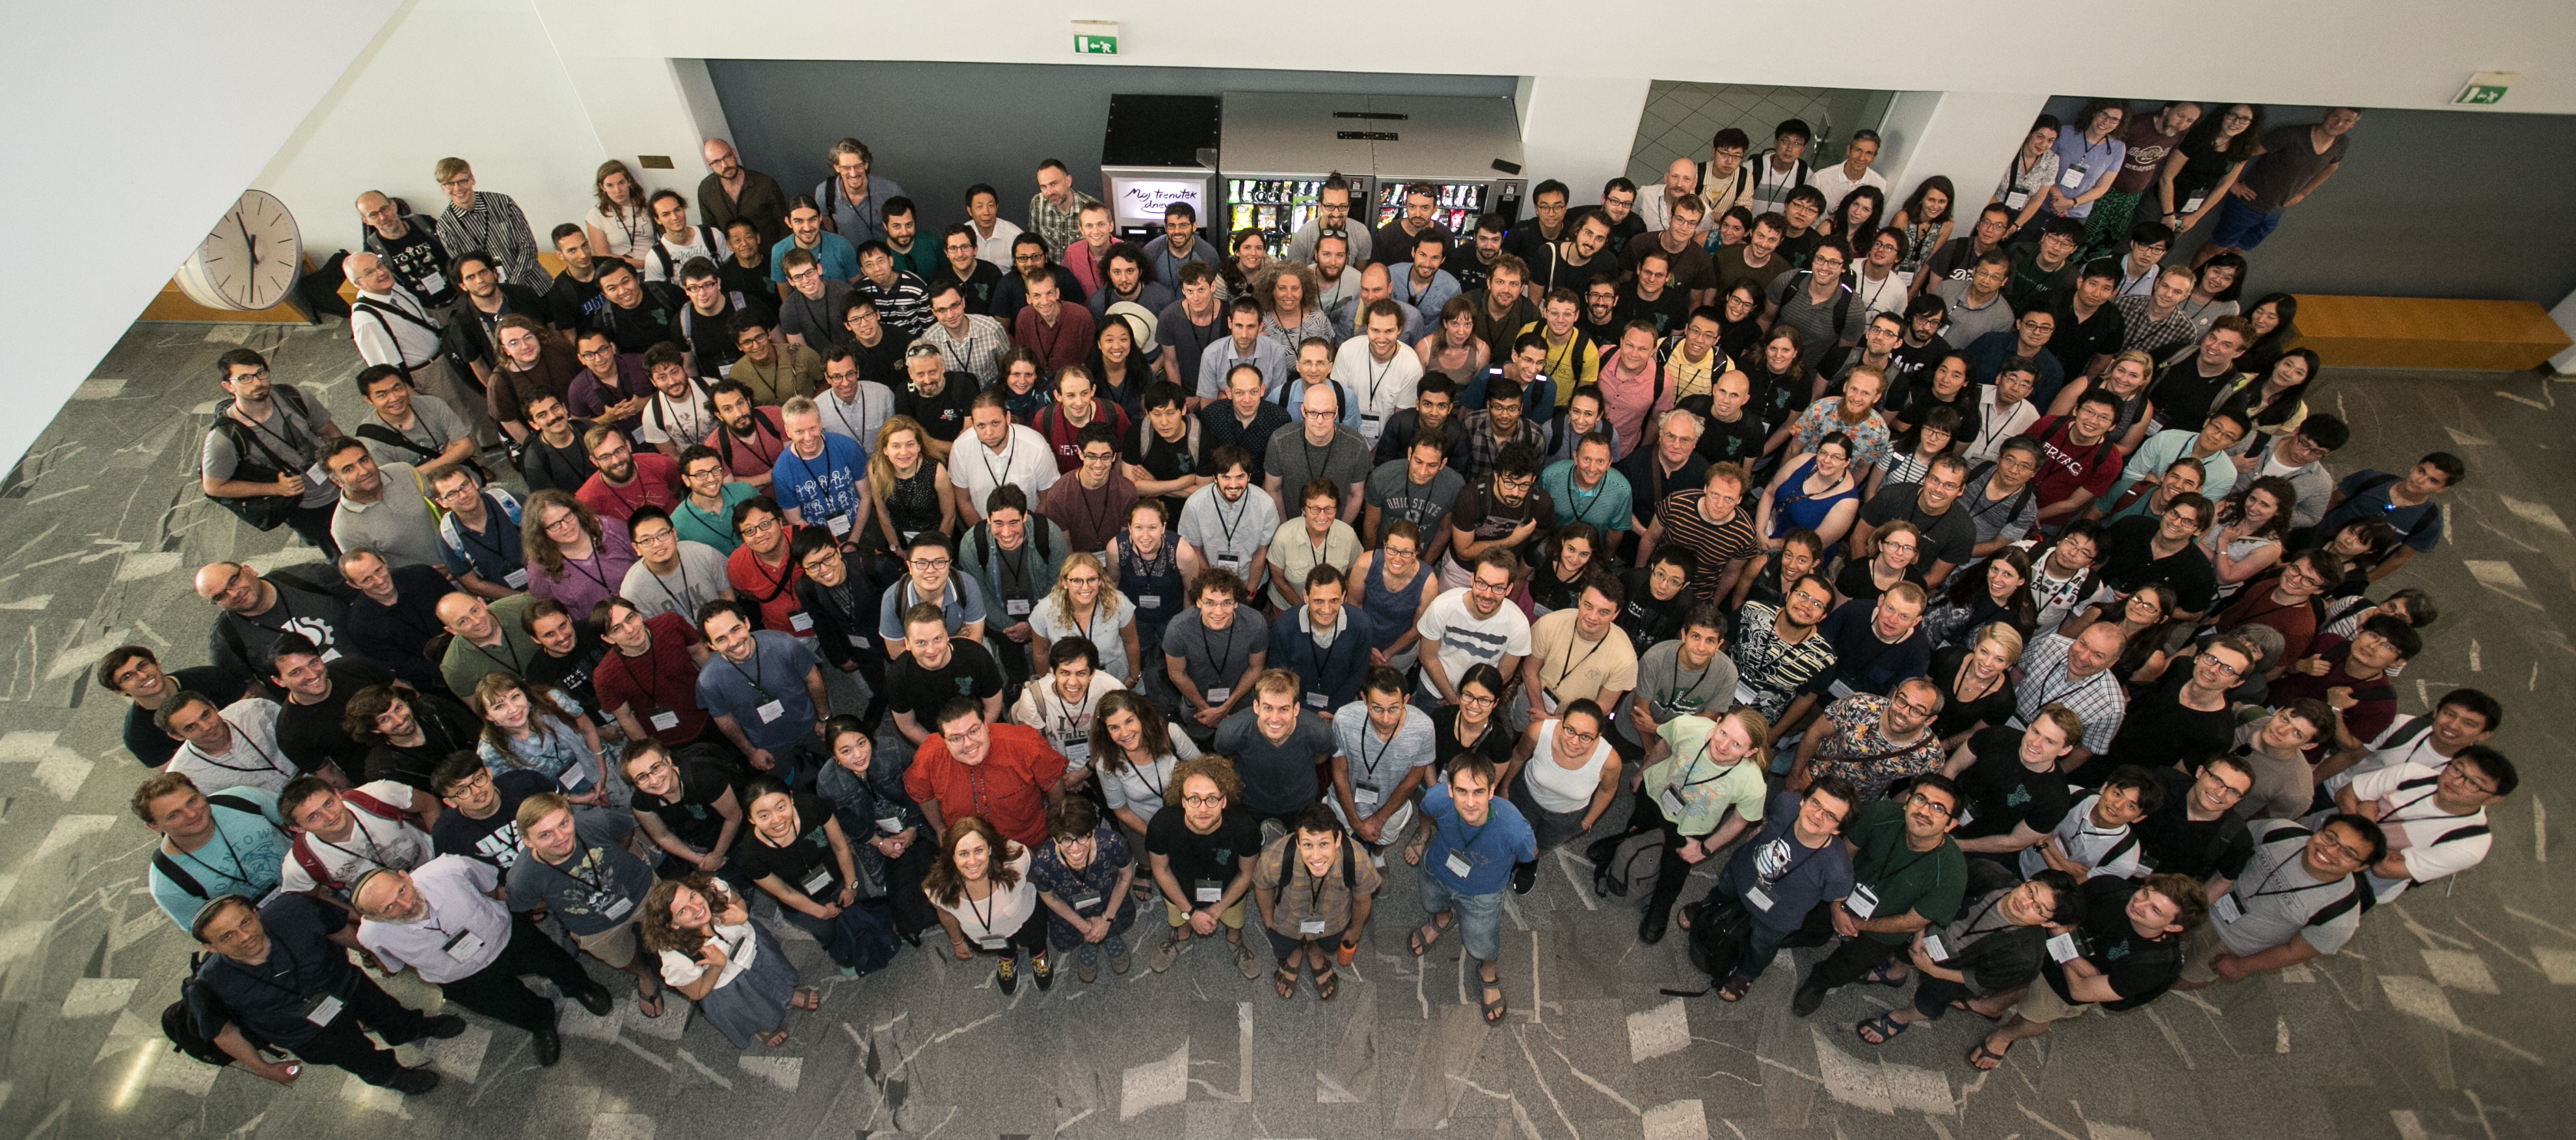
\includegraphics[scale=0.3]{FPSAC.jpg}
\caption*{International Conference on Formal Power Series and Algebraic Combinatorics, Ljubljana, Slovenia}
\end{figure}

\end{event}
